% Generated by make_fig_b_results.py from committed results. Do not edit by hand.
\documentclass[border=2pt]{standalone}
\usepackage[T1]{fontenc}\usepackage{newtxtext,newtxmath}\usepackage[varqu,scaled=0.95]{zi4}
\usepackage{pgfplots}\pgfplotsset{compat=1.18}\usepgfplotslibrary{groupplots}
\definecolor{cblue}{HTML}{0072B2}\definecolor{cver}{HTML}{D55E00}\definecolor{cora}{HTML}{E69F00}
\definecolor{cgreen}{HTML}{009E73}\definecolor{cgrey}{HTML}{999999}
\pgfplotsset{every axis/.append style={font=\footnotesize, tick label style={font=\scriptsize},
  label style={font=\footnotesize}, legend style={font=\scriptsize, draw=none, fill=none},
  axis lines*=left, grid style={black!8}}}
\begin{document}

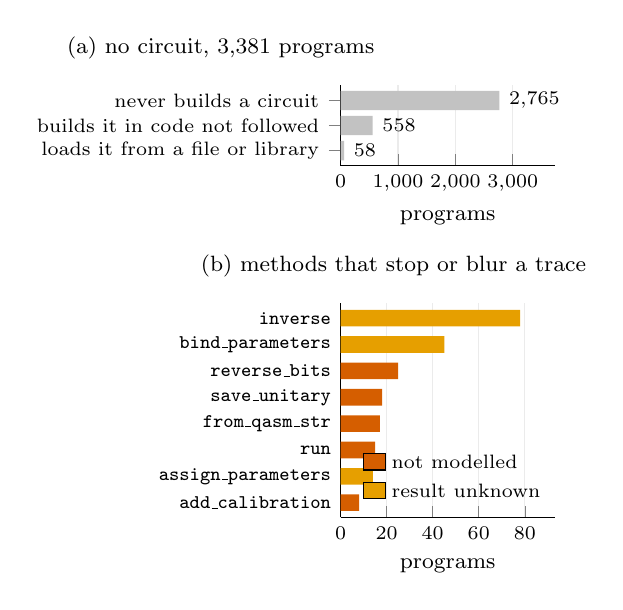
\begin{tikzpicture}
\begin{axis}[name=a, xbar, width=4.3cm, height=2.6cm, bar width=7pt, xmin=0, xmax=3732, symbolic y coords={{loads it from a file or library},{builds it in code not followed},{never builds a circuit}}, ytick=data, xmajorgrids, xlabel={programs}, nodes near coords, nodes near coords style={font=\scriptsize, anchor=west}, enlarge y limits=0.3, title={\footnotesize (a) no circuit, 3{,}381 programs}, title style={at={(0,1)}, anchor=south west, xshift=-3.6cm}]
\addplot[fill=cgrey!60, draw=none] coordinates {(2765,{never builds a circuit}) (558,{builds it in code not followed}) (58,{loads it from a file or library})};
\end{axis}
\begin{axis}[at={(a.south west)}, anchor=north west, yshift=-1.75cm, xbar stacked, width=4.3cm, height=4.3cm, bar width=6pt, xmin=0, xmax=93, symbolic y coords={{\texttt{add\_calibration}},{\texttt{assign\_parameters}},{\texttt{run}},{\texttt{from\_qasm\_str}},{\texttt{save\_unitary}},{\texttt{reverse\_bits}},{\texttt{bind\_parameters}},{\texttt{inverse}}}, ytick=data, xmajorgrids, xlabel={programs}, enlarge y limits=0.08, legend style={at={(1,0.02)}, anchor=south east, legend columns=1}, legend cell align=left, title={\footnotesize (b) methods that stop or blur a trace}, title style={at={(0,1)}, anchor=south west, xshift=-1.9cm}]
\addplot[fill=cver, draw=none] coordinates {(0,{\texttt{inverse}}) (0,{\texttt{bind\_parameters}}) (25,{\texttt{reverse\_bits}}) (18,{\texttt{save\_unitary}}) (17,{\texttt{from\_qasm\_str}}) (15,{\texttt{run}}) (0,{\texttt{assign\_parameters}}) (8,{\texttt{add\_calibration}})};
\addlegendentry{not modelled}
\addplot[fill=cora, draw=none] coordinates {(78,{\texttt{inverse}}) (45,{\texttt{bind\_parameters}}) (0,{\texttt{reverse\_bits}}) (0,{\texttt{save\_unitary}}) (0,{\texttt{from\_qasm\_str}}) (0,{\texttt{run}}) (14,{\texttt{assign\_parameters}}) (0,{\texttt{add\_calibration}})};
\addlegendentry{result unknown}
\end{axis}
\end{tikzpicture}
\end{document}
